\documentclass[bwprint]{gmcmthesis}
\usepackage{amsmath}
\usepackage{multirow}
\usepackage{threeparttable}
\numberwithin{figure}{section}
\renewcommand{\thefigure}{\arabic{section}-\arabic{figure}} 
\newcommand{\upcite}[1]{\textsuperscript{\textsuperscript{\cite{#1}}}}
% \documentclass[withoutpreface,bwprint]{cumcmthesis}
% 去掉封面与编号页

\title{中国研究生数学建模竞赛论文标题}
\baominghao{No.21104870023} %参赛队号
\schoolname{华中科技大学}%学校名称
\membera{张智璐} %队员A
\memberb{钱以骞} %队员B
\memberc{周鑫宜} %队员C
\begin{document}
 \maketitle
 \begin{abstract}
第一段:针对自己选择的题目,说明自己用了什么方法来解决的(这类题属于哪种典型的问题),其中利用了哪些关键的算法,再说出自己的所建模型的创新点。没有创新点,也可以说自己所建的模型相比较于其它的是一个很好的方案。

第二段:问题一中,针对具体问题,进行分析和求解,几句话介绍自己是怎么解决的,有数字结果的也可以直接贴结果。

第三段:问题二中,类比于第二段。

第四段:问题三中,类比于第三段。

第五段:问题四中,类比于第四段。

第六段:如果有问题五,类比于第五段,没有就结束,也可以写一下团队的想法。

随便加点东西






\keywords{针对具体的问题列一到两个关键字\quad  建模算法列出\quad }
\end{abstract}

%\pagestyle{plain}

%目录
\tableofcontents

\section{问题重述}
\subsection{问题背景}
环境空气污染能够对人类、动植物及产生较大的影响和危害。建立空气质量预报模型,提前预报大气污染状况能够支撑政府制定防治策略,提醒公众提前防范,减少自身暴露,减轻污染。

WRF-CMAQ模拟体系(以下简称WRF-CMAQ模型)是在 “一个大气” 理论的指导下,以WRF中尺度数值天气预报系统为依托,充分考虑了大气污染过程中水平传输、垂直传输、扩散过程、源排放、化学反应和去除过程等对污染物浓度的影响,将复杂空气污染状况进行综合处理\upcite{ref1}。WRF和CMAQ的结构如图\ref{fig1-1}和图\ref{fig1-2}所示。
\begin{figure}[!h]
	\centering
	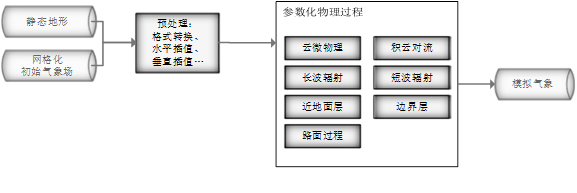
\includegraphics[width=.7\textwidth]{figures//fig1-1.png}
	\caption{中尺度数值天气预报系统WRF结构\upcite{ref2}}
	\label{fig1-1}
\end{figure}
\begin{figure}[!h]
	\centering
	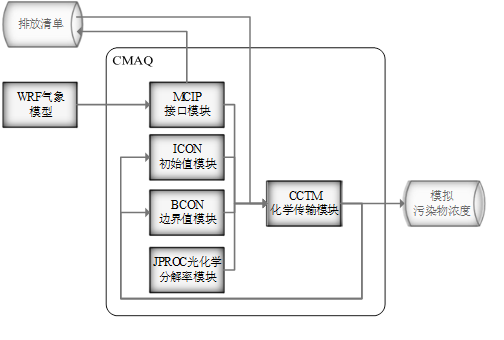
\includegraphics[width=.7\textwidth]{figures//fig1-2.png}
	\caption{空气质量预测与评估系统CMAQ结构\upcite{ref3}}
	\label{fig1-2}
\end{figure}

CMAQ是一种三维欧拉大气化学与传输模拟系统,经由对污染物变化过程的模拟得到具体时间点或时间段的预报结果,但由于模拟的气象场和排放清单的不确定性,同时还存在包括臭氧在内生成机理不完全明晰的污染物的存在,WRF-CMAQ预报模型的结果并不理想。为提高预报准确性,一种可行办法是在WRF-CMAQ等一次模型模拟结果的基础上,结合更多的数据源进行二次建模。二次模型与WRF-CMAQ模型关系如图\ref{fig1-3}所示。其中,由于气象条件对空气质量影响很大(例如湿度降低有利于臭氧的生成),且污染物浓度实测数据的变化情况对空气质量预报具有一定参考价值,因此实测数据源参考空气质量监测点获得的气象数据。
\begin{figure}[!h]
	\centering
	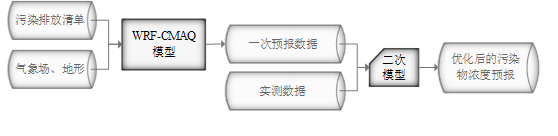
\includegraphics[width=.7\textwidth]{figures//fig1-3.png}
	\caption{空气质量预测与评估系统CMAQ结构}
	\label{fig1-3}
\end{figure}

\subsection{问题提出}
\textbf{问题1}使用附件1数据,计算监测点A从2020年8月25日到8月28日每天实测的AQI和首要污染物。

\textbf{问题2}使用附件1中的数据,根据对污染物浓度的影响程度,对气象条件进行合理分类,并阐述各类气象条件的特征。

\textbf{问题3}使用附件1和2的数据,建立适用3个监测点(忽略彼此影响)的二次预报数学模型,预测未来3天6种污染物浓度,要求预测结果AQI最大相对误差尽量小,首要污染物预测准确度尽量高。并用该模型预测ABC的2021年7月13到7月15的污染物浓度,计算AQI和首要污染物。

\textbf{问题4}使用附件1和3数据建立区域协同预报模型,包含A,A1,A2,A3四个监测点。要求预测结果AQI最大相对误差尽量小,首要污染物预测准确度尽量高。使用该协同预报模型预测监测点A、A1、A2、A3在2021年7月13日至7月15日的污染物浓度,计算AQI和首要污染物,并且讨论协同预报模型是否能提升准确度。

\begin{figure}[!h]
\centering
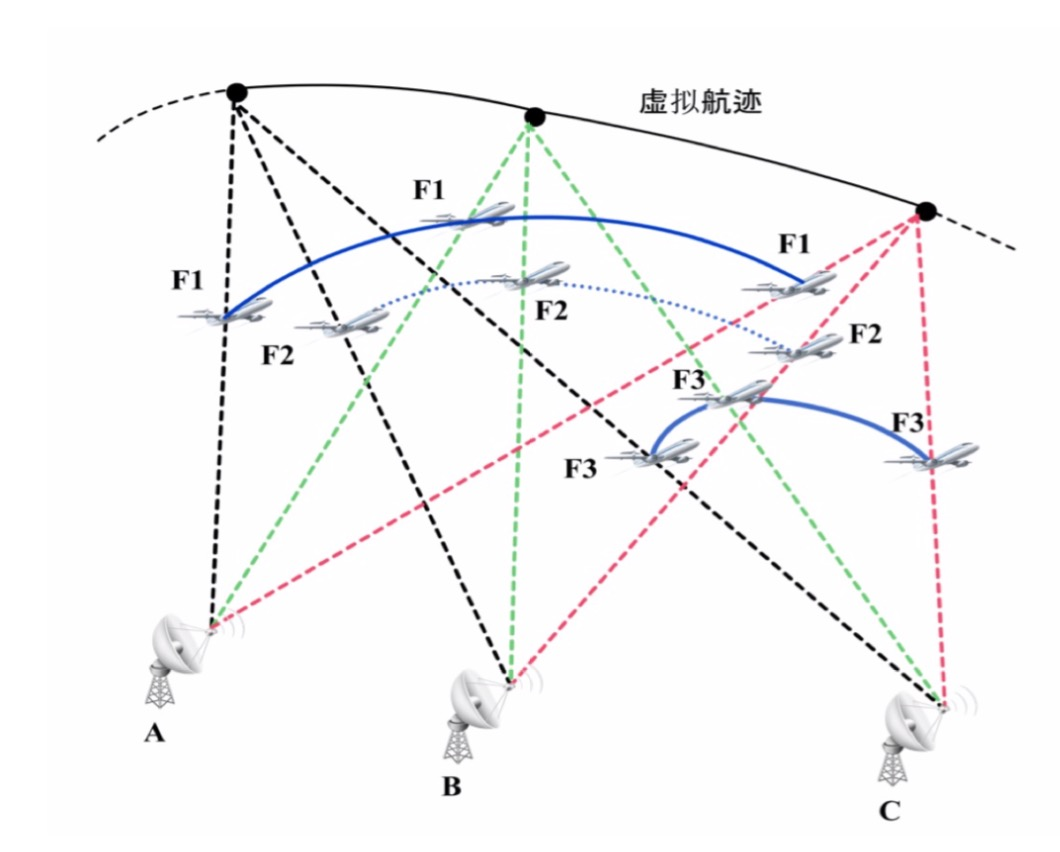
\includegraphics[width=.7\textwidth]{test.jpg}
\caption{对雷达实施距离多假目标欺骗干扰示意图}
\label{fig1}
\end{figure}
\begin{figure}[!h]
\centering
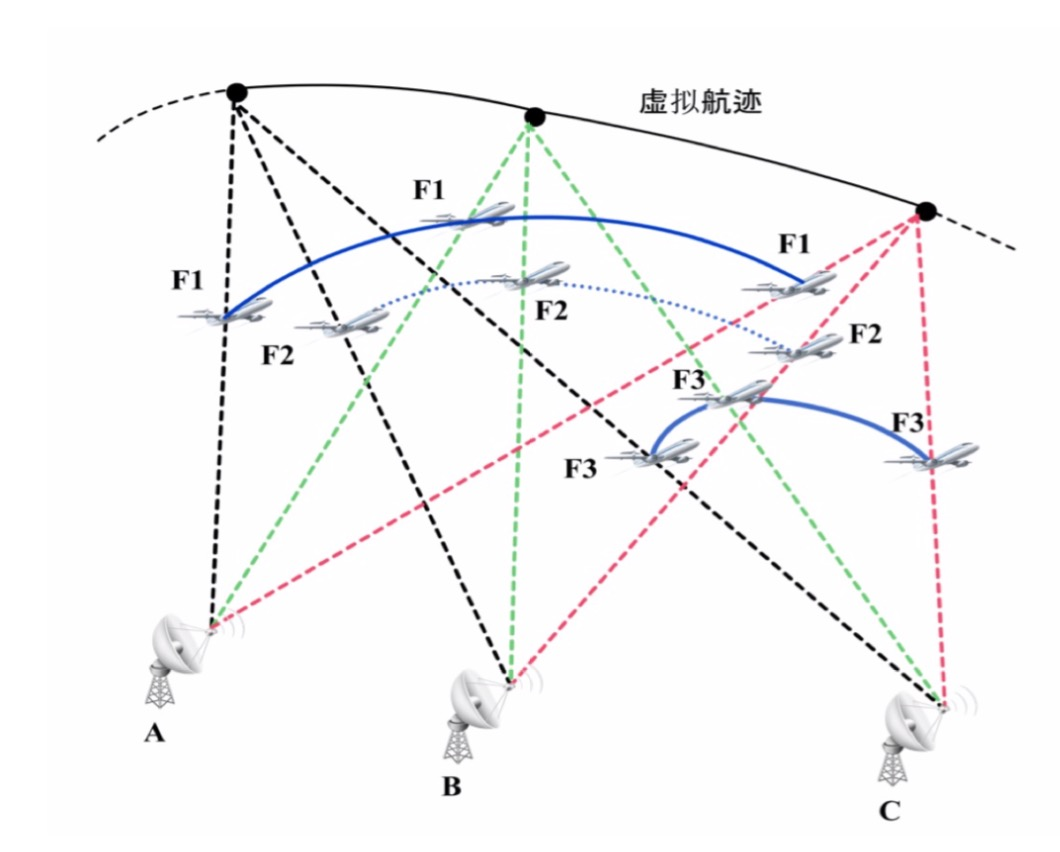
\includegraphics[width=.7\textwidth]{test.jpg}
\caption{对雷达实施距离多假目标欺骗干扰示意图}
\label{fig1}
\end{figure}

\section{模型假设}
模型假设模型假设模型假设模型假设模型假设模型假设模型假设模型假设模型假设模型假设模型假设模型假设模型假设模型假设模型假设模型假设模型假设模型假设。
\begin{figure}[!h]
\centering
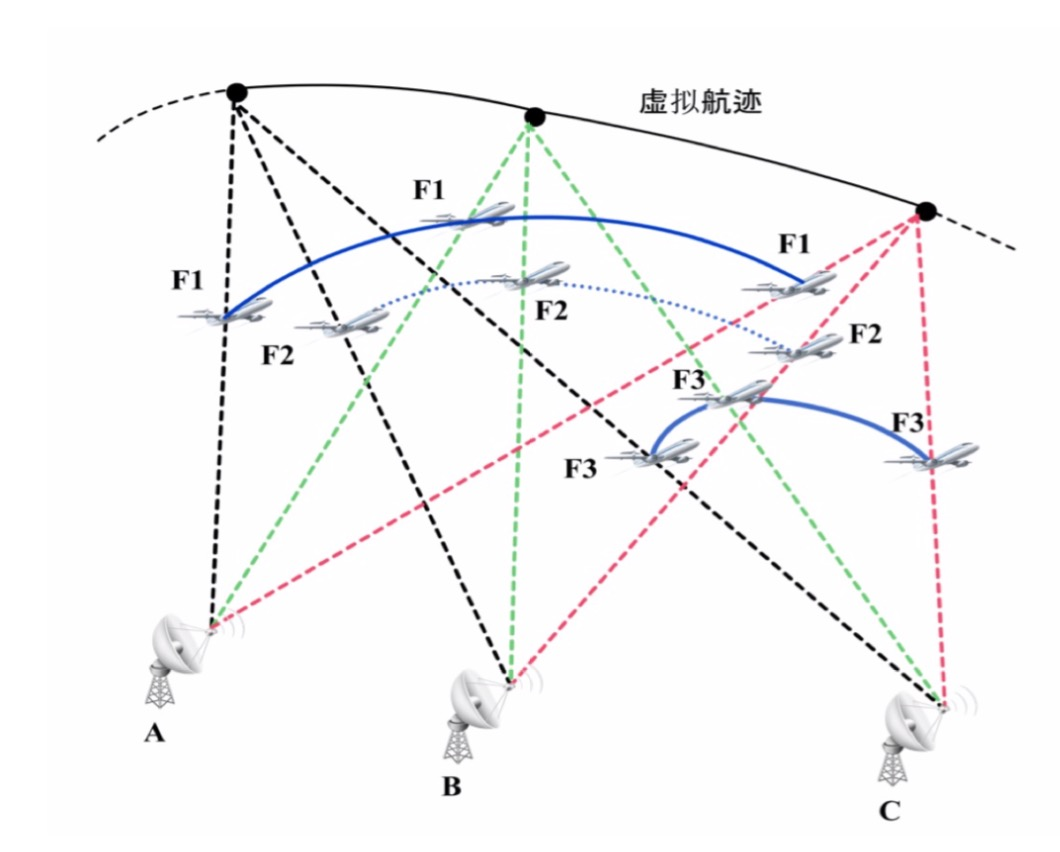
\includegraphics[width=.7\textwidth]{test.jpg}
\caption{对雷达实施距离多假目标欺骗干扰示意图}
\label{fig1}
\end{figure}

\begin{figure}[!h]
\centering
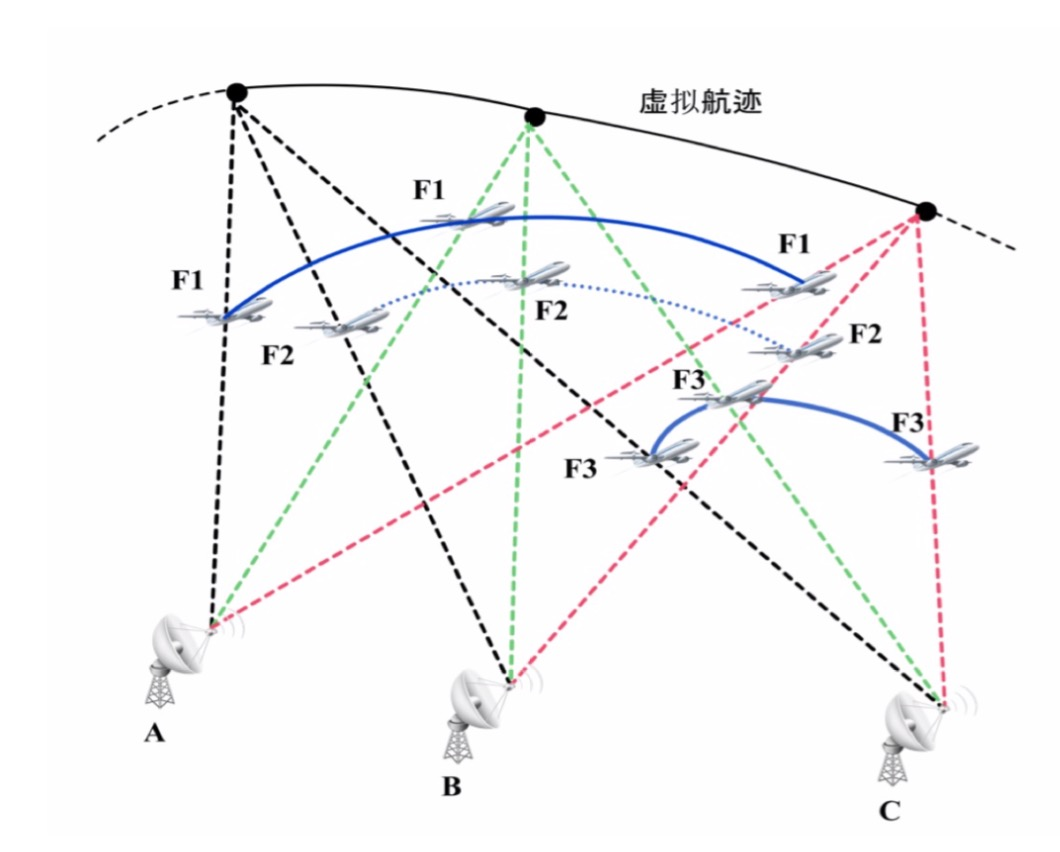
\includegraphics[width=.7\textwidth]{test.jpg}
\caption{对雷达实施距离多假目标欺骗干扰示意图}
\label{fig1}
\end{figure}

\begin{figure}[!h]
\centering
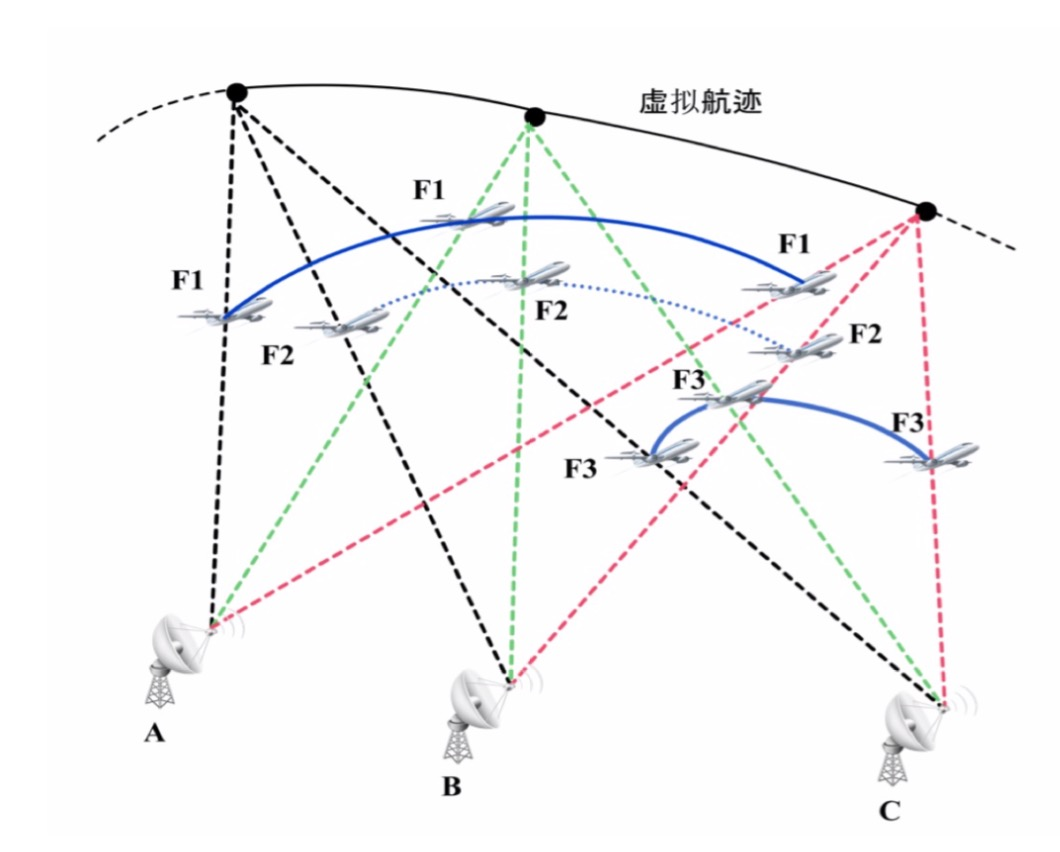
\includegraphics[width=.7\textwidth]{test.jpg}
\caption{对雷达实施距离多假目标欺骗干扰示意图}
\label{fig1}
\end{figure}
\section{符号说明}
符号说明符号说明符号说明符号说明符号说明符号说明符号说明符号说明符号说明符号说明符号说明符号说明符号说明符号说明符号说明符号说明符号说明。
\section{问题的分析}
\subsection{问题一的分析与求解}
\subsubsection{问题一的描述与分析}
问题一中提到的AQI即为空气质量指数,该数据可用于判别空气质量等级。AQI的计算方式如下:
首先需得到各项污染物的空气质量分指数(IAQI),其计算公式如公式(1)所示:
\begin{equation}
	\rm IAQI_P = \frac{IAQI_{Hi}-IAQI_{Lo}}{BP_{Hi}-BP_{Lo}}*(C_P-BP_{Lo})+IAQI_{Lo}
\end{equation}
式中各符号的含义如下:
\begin{itemize}
	\item $\rm IAQI_P$表示污染物P的空气质量分指数,结果进位取整数
	\item $\rm C_P$表示污染物P的质量浓度值
	\item $\rm BP_{Hi}, BP_{Lo}$表示与$\rm C_P$相近的污染物浓度限值的高位值与低位值
	\item $\rm IAQI_{Hi}, IAQI_{Lo}$表示与$\rm BP_{Hi},BP_{Lo}$对应的空气质量分指数
\end{itemize}

各项污染物项目浓度限值及对应的空气质量分指数级别见表\ref{tab:table4-1}:
\begin{table}[h!]
\caption{空气质量分指数(IAQI)及对应的污染物项目浓度限值}\label{tab:table4-1}
\begin{center}
\begin{threeparttable}
\resizebox{.95\columnwidth}{!}{
\begin{tabular}{|c|c|c|c|c|c|c|c|c|c|c|}
	\hline
	序号&指数或污染物项目&\multicolumn{8}{|c|}{空气质量分指数及对应污染物浓度限值}&单位 \\
	\hline
	0&空气质量分指数(IAQI)&0&50&100&150&200&300&400&500&-\\
	\hline
	1&一氧化碳(CO)24小时平均&0&2&4&14&24&36&48&60&$\rm mg∕m^3$\\
	\hline
	2&二氧化硫(SO2)24小时平均&0&50&150&475&800&1600&2100&2620&\multirow{5}{*}{$\rm μg∕m^3$} \\
	\cline{1-10}
	3&二氧化氮(NO2)24小时平均&0&40&80&180&280&565&750&940& \\
	\cline{1-10}
	4&臭氧(O3)最大8小时滑动平均&0&100&160&215&265&800&-&-& \\
	\cline{1-10}
	5&粒径小于等于10μm颗粒物
	(PM10)24小时平均&0&50&150&250&350&420&500&600& \\
	\cline{1-10}
	6&粒径小于等于2.5μm颗粒物
	(PM2.5)24小时平均&0&35&75&115&150&250&350&500& \\
	\hline
\end{tabular}
}
\begin{tablenotes}
	\footnotesize
	\item[1] 臭氧(O3)最大8小时滑动平均浓度值高于800 $\rm μg∕m^3$的,不再进行其空气质量分指数计算。
	\item[2] 其余污染物浓度高于IAQI=500对应限值时,不再进行其空气质量分指数计算
\end{tablenotes}
\end{threeparttable}      
\end{center}
\end{table}

空气质量指数(AQI)取各分指数中的最大值,即有
\begin{displaymath} 
	\rm AQI = max{IAQI_1,IAQI_2,...,IAQI_n}
\end{displaymath}
式中,$\rm IAQI_1,IAQI_2,IAQI_3,…,IAQI_n$为各污染物项目的分指数。在本题中,对于AQI的计算仅涉及表1提供的六种污染物,因此计算公式如公式(2)所示:
\begin{equation} 
	\rm AQI = max⁡{IAQI_{SO_2},IAQI_{NO_2},IAQI_{PM_10},IAQI_{PM_2.5},IAQI_{O_3},IAQI_CO}
\end{equation}
空气质量等级范围根据AQI数值划分,等级对应的AQI范围见表\ref{tab:table4-2}。
\begin{table}[h!]
	\caption{空气质量等级及对应空气质量指数(AQI)范围}\label{tab:table4-2}
	\begin{center}
		\begin{tabular}{|c|c|c|c|c|c|c|}
			\hline
			空气质量等级&优&良&轻度污染&中度污染&重度污染&严重污染 \\
			\hline
			空气质量指数(AQI)范围&[0,50]&[51,100]&[101,150]&[151,200]&[201,300]&[301,+∞) \\
			\hline
		\end{tabular}
	\end{center}
\end{table}

当AQI小于或等于50(即空气质量评价为“优”)时,称当天无首要污染物;
当AQI大于50时,IAQI最大的污染物为首要污染物。若IAQI最大的污染物为两项或两项以上时,并列为首要污染物
IAQI大于100的污染物为超标污染物。
则求解问题一需要根据附件1中提供的“监测点A逐日污染物浓度数据”表,通过上述方法计算监测点A从2020年8月25日到8月28日每天实测的AQI和首要污染物。
\subsubsection{问题一的求解}
问题一的求解过程较为简单,但是为了后期处理方便以及增强代码的可重用性,我们采用直接完全处理附件1中的“监测点A逐日污染物浓度数据”表的方式。在得到整个表的结果后,找出题目中的日期范围对应的结果。处理整个表格的流程图如\ref{fig4-1}所示:
\begin{figure}[!h]
	\centering
	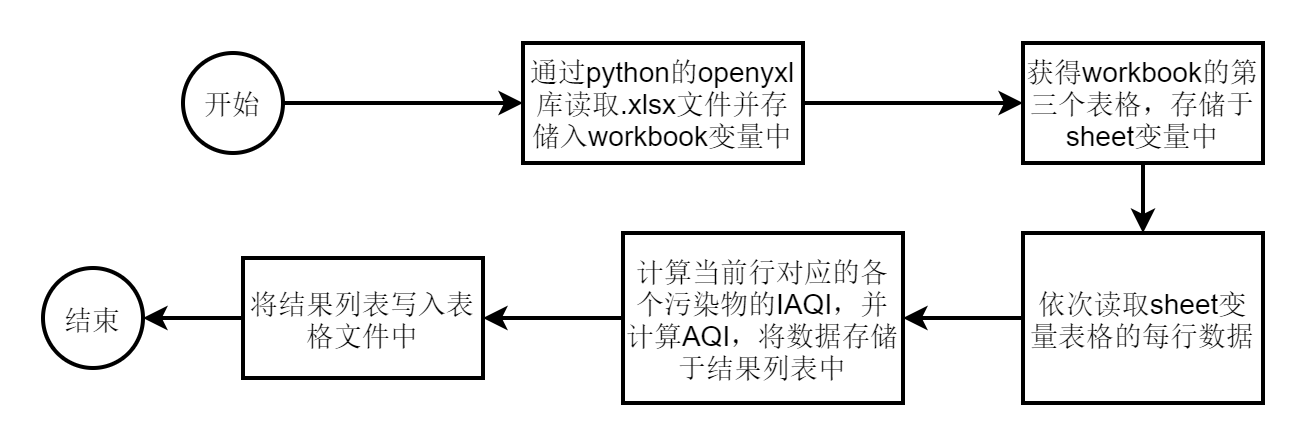
\includegraphics[width=.7\textwidth]{figures//fig4-1.png}
	\caption{完全处理“监测点A逐日污染物浓度数据”表流程图}
	\label{fig4-1}
\end{figure}

计算得到的结果如表\ref{tab:table4-3}所示
\begin{table}[h!]
	\caption{问题一AQI计算结果表}\label{tab:table4-3}
	\begin{center}
		\begin{tabular}{|c|c|c|c|}
			\hline
			\multirow{2}{*}{检测日期}&\multirow{2}{*}{地点}&\multicolumn{2}{|c|}{AQI计算} \\
			\cline{3-4}
			& &AQI&首要污染物\\
			\hline
			2020/8/25&监测点A&60&$\rm O_3$\\
			\hline
			2020/8/26&监测点A&46&无\\
			\hline
			2020/8/27&监测点A&109&$\rm O_3$\\
			\hline
			2020/8/28&监测点A&138&$\rm O_3$\\
			\hline
		\end{tabular}
	\end{center}
\end{table}

\subsection{问题二 xxx}
\subsubsection{问题描述和分析}
问题的分析问题的分析问题的分析问题的分析问题的分析问题的分析问题的分析问题的分析问题的分析问题的分析问题的分析问题的分析问题的分析问题的分析。
\subsubsection{模型建立与求解}
模型建立与求解模型建立与求解模型建立与求解模型建立与求解模型建立与求解模型建立与求解模型建立与求解模型建立与求解模型建立与求解模型建立与求解模型建立与求解。

\subsection{问题三 xxx}
\subsubsection{问题描述和分析}
问题的分析问题的分析问题的分析问题的分析问题的分析问题的分析问题的分析问题的分析问题的分析问题的分析问题的分析问题的分析问题的分析问题的分析。
\subsubsection{模型建立与求解}
模型建立与求解模型建立与求解模型建立与求解模型建立与求解模型建立与求解模型建立与求解模型建立与求解模型建立与求解模型建立与求解模型建立与求解模型建立与求解。

\subsection{问题四 xxx}
\subsubsection{问题描述和分析}
问题的分析问题的分析问题的分析问题的分析问题的分析问题的分析问题的分析问题的分析问题的分析问题的分析问题的分析问题的分析问题的分析问题的分析。
\subsubsection{模型建立与求解}
模型建立与求解模型建立与求解模型建立与求解模型建立与求解模型建立与求解模型建立与求解模型建立与求解模型建立与求解模型建立与求解模型建立与求解模型建立与求解。

\section{模型的评价}
\subsection{模型的优点}
模型的优点模型的优点模型的优点模型的优点模型的优点模型的优点模型的优点模型的优点模型的优点模型的优点模型的优点模型的优点模型的优点模型的优点。
\subsection{模型的缺点}
模型的缺点模型的缺点模型的缺点模型的缺点模型的缺点模型的缺点模型的缺点模型的缺点模型的缺点模型的缺点模型的缺点模型的缺点模型的缺点模型的缺点。



\section{写作参考格式}
写作过程中可能要用到一些格式参考,正式写作的时候,可以直接将这一章删掉即可。

\textbf{无序列表格式}
\begin{itemize}
\item 无序列表1
\item 无序列表2
\item 无序列表3
\item 无序列表4
\end{itemize}


\textbf{表格格式}

\begin{tabular}{cc}
 \hline
 \makebox[0.4\textwidth][c]{符号}	&  \makebox[0.5\textwidth][c]{意义} \\ \hline
 D	    & 宽度(cm) \\ \hline
 L	    & 长度(cm)  \\ \hline
\end{tabular}


%
%\textbf{图片格式}
%\begin{figure}[h]
%\centering
%\includegraphics[width=5cm]{xxx.jpg}
%\caption{图片标题}
%\end{figure}

\section{参考文献}
%参考文献
\begin{thebibliography}{1.2}%宽度9
\setlength{\itemsep}{-2mm}
 \bibitem{ref1}
 宋鹏程, 张馨文, 黄强, 等. 我国城市环境空气质量预报主要模型及应用[J]. 四川环境, 2019, 3.
 \bibitem{ref2}
 伯鑫 等. 空气质量模型(SMOKE、WRF、CMAQ等)操作指南及案例研究 [M]. 北京: 中国环境出版集团, 2019.
 \bibitem{ref3}
 戴树桂. 环境化学 [M]. 北京: 高等教育出版社, 1997.
 \bibitem{ref4}
 赵秋月, 李荔, 李慧鹏. 国内外近地面臭氧污染研究进展 [J]. 环境科技, 2018, 31(05): 72-76.
 \bibitem{ref5}
 陈敏东. 大气臭氧污染形成机制及研究进展 [J/OL] 2018, https://max.book118.com/html/2018/0201/151478594.shtm. 
\end{thebibliography}

\newpage
%附录
\appendix
\section{程序代码}
%设置不同语言即可。
\begin{lstlisting}[language=Matlab] 
kk=2;[mdd,ndd]=size(dd);
while ~isempty(V)
[tmpd,j]=min(W(i,V));tmpj=V(j);
for k=2:ndd
[tmp1,jj]=min(dd(1,k)+W(dd(2,k),V));
tmp2=V(jj);tt(k-1,:)=[tmp1,tmp2,jj];
end
tmp=[tmpd,tmpj,j;tt];[tmp3,tmp4]=min(tmp(:,1));
if tmp3==tmpd, ss(1:2,kk)=[i;tmp(tmp4,2)];
else,tmp5=find(ss(:,tmp4)~=0);tmp6=length(tmp5);
if dd(2,tmp4)==ss(tmp6,tmp4)
ss(1:tmp6+1,kk)=[ss(tmp5,tmp4);tmp(tmp4,2)];
else, ss(1:3,kk)=[i;dd(2,tmp4);tmp(tmp4,2)];
end;end
dd=[dd,[tmp3;tmp(tmp4,2)]];V(tmp(tmp4,3))=[];
[mdd,ndd]=size(dd);kk=kk+1;
end; S=ss; D=dd(1,:);
 \end{lstlisting}


\end{document} 